%TC:ignore
\begin{table}[H]
    \caption{Results on Gowalla instances}\label{table:gowalla_cost}
    \tiny
    \begin{tabularx}{\textwidth}{llXXXXlXXXXlXX}
    \firsthline
    \multicolumn{1}{c}{Instance}& \quad & \multicolumn{4}{c}{Pseudo $O(1)-approximation$}& \quad & \multicolumn{4}{c}{Colourful PBS} & \quad & \multicolumn{2}{c}{Statistics}\\
    \cline{1-1} \cline{3-6} \cline{8-11} \cline{13-14}\\
    name && min & $\mu$ & $\sigma$ & $\mu (time)$ && min & $\mu$ & $\sigma$ & $\mu (time)$ && \%-gap (cost) & \%-gap (time)\\
    \hline
    gow01 && 38.07 & 38.07 & 0.00 & 1.88 && 12.39 & 12.46 & 0.15 & 7.39 && -67.29 & 293.90\\
    gow02 && 2.27 & 2.27 & 0.00 & 1.80 && 1.11 & 1.13 & 0.00 & 6.50 && -50.18 & 261.76\\
    gow03 && 22.74 & 22.74 & 0.00 & 1.84 && 11.28 & 11.36 & 0.03 & 4.32 && -50.07 & 135.08\\
    gow04 && 2.70 & 2.70 & 0.00 & 0.85 && 1.35 & 1.35 & 0.00 & 3.27 && -50.00 & 282.54\\
    gow05 && 1.72 & 1.72 & 0.00 & 0.91 && 0.86 & 0.91 & 0.04 & 12.77 && -47.45 & 1301.59\\
    gow06 && 774.60 & 774.60 & 0.00 & 4.78 && 277.88 & 277.88 & 0.00 & 9.80 && -64.13 & 104.98\\
    gow07 && 52.34 & 52.34 & 0.00 & 2.11 && 26.46 & 26.50 & 0.23 & 8.65 && -49.38 & 310.12\\
    gow08 && 4.07 & 4.07 & 0.00 & 2.05 && 2.04 & 2.06 & 0.06 & 12.75 && -49.33 & 522.86\\
    gow09 && 4.19 & 4.19 & 0.00 & 1.97 && 2.10 & 2.17 & 0.04 & 24.10 && -48.13 & 1121.91\\
    gow10 && 1.32 & 1.32 & 0.00 & 1.96 && 0.75 & 0.80 & 0.02 & 34.81 && -39.48 & 1680.46\\
    gow11 && 1050.87 & 1050.87 & 0.00 & 9.23 && 495.18 & 509.63 & 2.96 & 18.94 && -51.50 & 105.04\\
    gow12 && 54.53 & 54.53 & 0.00 & 4.12 && 29.21 & 30.10 & 1.21 & 26.71 && -44.81 & 548.66\\
    gow13 && 9.80 & 9.80 & 0.00 & 3.69 && 4.94 & 5.61 & 0.39 & 29.28 && -42.78 & 693.81\\
    gow14 && 0.58 & 0.58 & 0.00 & 3.80 && 0.33 & 0.37 & 0.02 & 37.77 && -35.74 & 894.99\\
    gow15 && 2.59 & 2.59 & 0.00 & 3.84 && 1.39 & 1.75 & 0.19 & 37.20 && -32.46 & 869.05\\
    gow16 && 801.69 & 801.69 & 0.00 & 7.42 && 400.84 & 420.88 & 29.99 & 29.76 && -47.50 & 300.84\\
    gow17 && 379.08 & 379.08 & 0.00 & 12.93 && 188.74 & 189.19 & 1.34 & 42.57 && -50.09 & 229.22\\
    gow18 && 28.53 & 28.53 & 0.00 & 5.82 && 15.25 & 16.48 & 0.68 & 44.33 && -42.24 & 662.26\\
    gow19 && 6.49 & 6.49 & 0.00 & 5.72 && 3.28 & 3.67 & 0.14 & 52.57 && -43.43 & 818.83\\
    gow20 && 0.97 & 0.97 & 0.00 & 11.76 && 0.55 & 0.72 & 0.06 & 70.25 && -26.05 & 497.40\\
    gow21 && 898.02 & 898.02 & 0.00 & 21.39 && 308.76 & 351.59 & 22.84 & 51.36 && -60.85 & 140.15\\
    gow22 && 550.80 & 550.80 & 0.00 & 19.45 && 233.02 & 273.23 & 12.39 & 54.18 && -50.39 & 178.51\\
    gow23 && 16.65 & 16.65 & 0.00 & 8.75 && 8.54 & 9.07 & 0.89 & 55.69 && -45.56 & 536.39\\
    gow24 && 3.52 & 3.52 & 0.00 & 8.79 && 2.05 & 2.45 & 0.21 & 76.69 && -30.22 & 772.47\\
    gow25 && 1.31 & 1.31 & 0.00 & 17.73 && 0.77 & 0.92 & 0.08 & 74.68 && -29.60 & 321.26\\
    gow26 && 1038.79 & 1038.79 & 0.00 & 32.02 && 422.87 & 472.10 & 46.67 & 62.11 && -54.55 & 93.96\\
    gow27 && 341.32 & 341.32 & 0.00 & 27.08 && 170.29 & 205.67 & 29.69 & 61.28 && -39.74 & 126.32\\
    gow28 && 14.66 & 14.66 & 0.00 & 24.17 && 8.21 & 9.42 & 0.50 & 88.43 && -35.79 & 265.91\\
    gow29 && 3.46 & 3.46 & 0.00 & 24.29 && 1.96 & 2.24 & 0.23 & 104.95 && -35.27 & 332.02\\
    gow30 && 1.14 & 1.14 & 0.00 & 25.19 && 0.70 & 0.84 & 0.10 & 113.78 && -26.32 & 351.70\\
    gow31 && 1365.06 & 1365.06 & 0.00 & 44.23 && 523.64 & 658.87 & 56.73 & 76.46 && -51.73 & 72.88\\
    gow32 && 561.62 & 561.62 & 0.00 & 37.48 && 279.51 & 354.45 & 27.06 & 78.87 && -36.89 & 110.42\\
    gow33 && 11.52 & 11.52 & 0.00 & 34.83 && 6.70 & 8.02 & 1.31 & 108.16 && -30.40 & 210.58\\
    gow34 && 3.99 & 3.99 & 0.00 & 33.03 && 2.21 & 2.72 & 0.31 & 123.28 && -31.81 & 273.19\\
    gow35 && 1107.44 & 1107.44 & 0.00 & 25.69 && 554.25 & 708.06 & 97.53 & 75.15 && -36.06 & 192.51\\
    gow36 && 665.00 & 665.00 & 0.00 & 23.77 && 351.33 & 367.60 & 4.13 & 37.48 && -44.72 & 57.70\\
    gow37 && 645.74 & 645.74 & 0.00 & 24.45 && 334.58 & 396.61 & 26.57 & 75.02 && -38.58 & 206.78\\
    gow38 && 1161.61 & 1161.61 & 0.00 & 33.77 && 585.38 & 665.95 & 22.44 & 65.17 && -42.67 & 92.99\\
    gow39 && 618.42 & 618.42 & 0.00 & 60.81 && 277.00 & 357.25 & 39.18 & 93.95 && -42.23 & 54.50\\
    gow40 && 18.18 & 18.18 & 0.00 & 55.67 && 10.54 & 12.29 & 1.40 & 140.04 && -32.42 & 151.58\\
    \hline
    \multicolumn{1}{l}{Average} &&& 306.69 && 16.78 &&& 159.36 && 53.26 && -43.20 & 404.43\\
    \hline
    \multicolumn{5}{l}{Wilcoxon Signed Rank Test on mean costs:} & \multicolumn{9}{l}{p-value=\num{1.819e-12}}\\
        \lasthline
    \end{tabularx}
    \normalsize
\end{table}
%TC:endignore

\paragraph{Analysis of solution cost}~\\
Our result for the Wilcoxon test (\Cref{method:wilcoxon_test}) was \num{1.819e-12}, proving our observations to be statistically significant. From analysis using \Cref{method:counting_results}, colourful PBS produced lower costs than the \emph{Ban} algorithm for all 40 instances. The mean cost was 43.2\% lower on average.

To account for variance we conduct analysis using \Cref{method:counting_results_variance}. Using $\Delta =2$, which accounts for 95\% of the distribution, colorful \acrshort{pbs} outperforms \emph{Ban} for all 40 Gowalla problems. Furthermore if we take $\Delta =3$, which accounts for 99.7\% of the distribution, our algorithm still has lower costs for 39/40 problem instances.

\paragraph{Further analysis}~\\
We ran the brute force algorithm (\cref{alg:brute_force_colourful_k_center}) to obtain an optimal solution of a smaller 55 node problem instance (this took 5 hours and 16 minutes).

%TC:ignore
\begin{table}[H]
    \centering
    \tiny
    \caption{Performance on real world problem instance (gow41) with known optimal solution}
    \begin{tabular}{cccccccccccccccccc}
        \firsthline
        \multicolumn{4}{c}{Graph Details} & & \multicolumn{3}{c}{Constraints} & & \multicolumn{1}{c}{Optimal solution} & & \multicolumn{3}{c}{\emph{Ban} algorithm} & & \multicolumn{3}{c}{Colourful PBS}\\
        \cline{1-4} \cline{6-8} \cline{10-10} \cline{12-14} \cline{16-18}\\
         name &  n & blue & red & & k & min red & min blue & & optimal cost & & $\mu$ & $\sigma$ & \%-gap (opt) & & $\mu$ & $\sigma$ & \%-gap (opt)\\
         \hline
        gow41 & 55 & 15 & 40 & & 5 & 11 & 30 & & 577.26 & & 1089.92 & 0.00 & 88.81 & & 577.26 & 0.00 & 0.00\\
        \lasthline
    \end{tabular}
    \label{tab:brute_force_gowalla}
    \normalsize
\end{table}
%TC:endignore

Over 50 trials, colourful PBS converges to the optimal cost without fail whereas the \emph{Ban} algorithm achieves a cost 80\% above the optimal.

\begin{figure}[H]
    \centering
    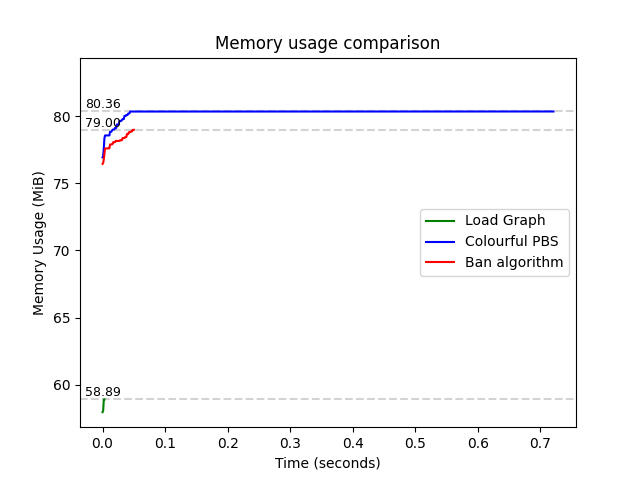
\includegraphics[width=0.7\textwidth]{images/memory_usage.png}
    \caption{Comparison of memory usage on gow41 problem instance\\ (dotted line indicates peak memory usage)}
    \label{fig:memory_usage}
\end{figure}

Analysing memory usage (\cref{fig:memory_usage}), colourful PBS uses 1.7\% more memory than \emph{Ban}, however this is insignificant compared to the memory required to store the graph which is around ~70\% of memory usage for both algorithms .

Overall for the real word 3D Gowalla data set Colourful PBS produces better results than the \emph{Ban} algorithm even after accounting for variance, however on average it incurs a five-fold increase in runtime.